\documentclass[acmlarge,screen,nonacm]{acmart}

% --- packages not already loaded by acmart ---
\usepackage{tabularx}

% suppress the ACM reference block (also implied by nonacm)
\settopmatter{printacmref=false}
\setlength{\footskip}{12pt}

% --- float placement tuning -------------------------------------------
% The defaults are conservative (topfraction 0.7, totalnumber 3), which
% causes tall figures restricted to [t] to be deferred and pile up at the
% end of the document. Loosening these lets figures sit near their text.
\renewcommand{\topfraction}{0.9}        % up to 90% of a page top can be floats
\renewcommand{\bottomfraction}{0.9}     % same for the bottom
\renewcommand{\textfraction}{0.07}      % require very little text per page
\renewcommand{\floatpagefraction}{0.7}  % a float page must be >=70% full
\setcounter{topnumber}{3}               % allow more floats at the top
\setcounter{bottomnumber}{3}            % and at the bottom
\setcounter{totalnumber}{5}             % and more floats overall per page

% Tighten the whitespace LaTeX inserts around floats to reclaim vertical space.
\setlength{\textfloatsep}{8pt plus 2pt minus 2pt}
\setlength{\floatsep}{8pt plus 2pt minus 2pt}
\setlength{\intextsep}{8pt plus 2pt minus 2pt}


%=====================================================================
\begin{document}

\title{Tactile Hands: A Force-Sensing Robotic Hand for Safe Grasping}

\author{Bryce Hackel}
\affiliation{%
  \institution{University of California, San Diego}
  \city{La Jolla}\state{California}\country{USA}}
\email{bhackel@ucsd.edu}

\author{Ali El Lahib}
\affiliation{%
  \institution{University of California, San Diego}
  \city{La Jolla}\state{California}\country{USA}}
\email{aellahib@ucsd.edu}

\author{Thomas Nghiem}
\affiliation{%
  \institution{University of California, San Diego}
  \city{La Jolla}\state{California}\country{USA}}
\email{tnghiem@ucsd.edu}

\author{Shree Venkatesh}
\affiliation{%
  \institution{University of California, San Diego}
  \city{La Jolla}\state{California}\country{USA}}
\email{s1venkatesh@ucsd.edu}

\author{Sidath Daham Wijesinghe}
\affiliation{%
  \institution{University of California, San Diego}
  \city{La Jolla}\state{California}\country{USA}}
\email{swijesinghe@ucsd.edu}

\renewcommand{\shortauthors}{Triton Droids: Tactile Hands}

\begin{abstract}
Robotic hands that grasp without sensing how hard they squeeze can crush
fragile objects, yet no open-source hand under \$200 offers fingertip force
sensing. We present Tactile Hands, a sub-\$200, four-fingered robotic hand that
adds calibrated fingertip force-sensing resistors (FSRs) to the open-source
AmazingHand. A custom ESP32-S3 board reads four FSRs through voltage dividers
and streams calibrated forces to a ROS~2 host, where a force-aware controller
halts finger closure at a safe threshold. Calibration reaches better-than-1~N
accuracy. Mounted on a teleoperated arm and driven in VR, the same controller
grasps a thin-walled cup without crushing it, where a force-blind grasp collapses
it. Our work presents a low-cost foundation for researchers and hobbyists to perform tactile manipulation.
\end{abstract}

\keywords{tactile sensing, force-sensing resistors, robotic hand, grasping,
calibration, teleoperation, ROS~2, low-cost robotics}

\maketitle

%=====================================================================
\section{Introduction}
%=====================================================================
A robot arm can be precise to the millimeter and still be dangerous, because
position tells it nothing about force. A hand that cannot feel how hard it is
gripping will crush a paper cup as readily as it lifts a steel block.
Humans avoid this with fingertip touch that modulates grip in real time;
bringing the same fingertip force sensing to robots is what separates a hand
that ``closes until it stops'' from one that ``closes until it feels enough.''

High-end research hands such as the Shadow Dexterous Hand or sensorized hands
built around GelSight~\cite{yuan2017gelsight} and DIGIT~\cite{lambeta2020digit}
tactile sensors demonstrate the value of touch, but they cost thousands of
dollars and are out of reach for most students and small labs.
Low-cost open-source hands have begun to close this gap on the mechanical side:
the LEAP Hand~\cite{shaw2023leap} and the AmazingHand~\cite{pollen2025amazinghand}
are anthropomorphic, 3D-printable, and affordable. However, these affordable
platforms ship without fingertip force sensing. To our knowledge, there is no
open-source robotic hand available for under roughly \$200 that provides
calibrated fingertip force measurement and uses it to grasp safely. This is the
gap our project targets.

Why is this capability missing at low cost? High-fidelity tactile sensors are
expensive (Section~\ref{sec:related}), whereas force-sensing resistors (FSRs)
cost a few dollars each, need a single analog channel, and add no per-finger
compute. Their drawback is
signal quality: FSRs are nonlinear, hysteretic, and vary unit to unit, so a raw
reading is not a force. We treated this as an engineering problem rather than a
fundamental limit. With a controlled calibration procedure and a simple
per-sensor model, inexpensive FSRs can be made accurate enough (better than
1~N) to close a useful safety loop, which is all that grasping a fragile object
without crushing it actually requires.

We present \textbf{Tactile Hands}, a four-fingered robotic hand built on the
open-source AmazingHand mechanical platform and augmented with a fingertip
force-sensing subsystem of our own design. Each fingertip carries a
force-sensing resistor (FSR); a custom ESP32-S3 board reads all four sensors
through voltage dividers, converts raw ADC readings to Newtons using a
calibrated power-law model, and streams the values over USB to a ROS~2 host. A
force-aware grasp controller continuously compares each fingertip force against
a safe threshold and stops closing a finger the moment that threshold is
crossed, allowing the hand to wrap a thin-walled paper cup and hold it without
collapsing it. The complete bill of materials remains under \$200. That figure
covers the hand itself driven by a laptop webcam; the Valve Index controllers
and ARCTOS arm are stretch additions on top.

Beyond the core force-sensing minimum viable product (MVP), we built three
input and simulation extensions that share the same ROS~2 backbone: a
webcam-based hand-pose pipeline that mirrors a human operator's finger curl onto
the hand, a physics simulation of the AmazingHand for kinematics validation and
future sim-to-real work, and a virtual-reality (VR) teleoperation pipeline that
streams 6-DoF controller pose into ROS~2. Most recently, we mounted the hand on
an open-source ARCTOS robotic arm~\cite{arctos2024} and teleoperated its
end-effector from VR controllers (Section~\ref{sec:teleopgrasp}). We
further added vision-guided, multi-object grip selection: a fine-tuned YOLO26
object detector recognizes the target object in a webcam image and selects an
appropriate per-object grip force automatically.

\paragraph{Contributions.} This paper makes the following contributions:
\begin{itemize}
  \item A \textbf{sub-\$200, open hardware design} that adds fingertip force
        sensing to a low-cost, 3D-printable robotic hand, including a custom
        ESP32-S3 sensing board with per-channel voltage dividers.
  \item A \textbf{repeatable FSR calibration procedure} using stacked 3D-printed
        reference weights and a power-law fit that maps raw ADC counts to force
        with better-than-1~N accuracy (max error 25.7~g $\approx$ 0.25~N).
  \item A \textbf{force-aware grasp controller} on a ROS~2 host that fuses the
        calibrated fingertip forces with finger position commands to grasp and
        release a fragile object without crushing it.
  \item A \textbf{teleoperation demonstration of the force-aware safety}: using VR control of the arm-mounted hand, force-thresholded
        grasping holds a fragile cup that an otherwise-identical force-blind
        grasp visibly collapses, showing the contribution of the tactile
        feedback.
  \item A set of \textbf{teleoperation and simulation extensions}
        (webcam hand-pose mirroring, physics simulation, and VR controller
        streaming) that share one ROS~2 interface, culminating in a
        VR-teleoperated, arm-mounted hand and a vision-guided, multi-object
        grip-selection pipeline driven by a fine-tuned YOLO26 detector.
\end{itemize}

The remainder of the paper reviews related work
(Section~\ref{sec:related}), details the system design and each subsystem
(Section~\ref{sec:technical}), reports our milestone history including
mid-quarter revisions and the problems we encountered
(Section~\ref{sec:milestones}), and concludes with future work
(Section~\ref{sec:conclusion}).

%=====================================================================
\section{Related Works}
\label{sec:related}
%=====================================================================
Our project sits at the intersection of low-cost robot hands, tactile sensing,
and teleoperation. We summarize the most relevant prior work in each area and
explain how Tactile Hands relates to it.

\paragraph{Low-cost and open-source robotic hands.}
The LEAP Hand~\cite{shaw2023leap} demonstrated that an anthropomorphic,
dexterous hand can be built for a few hundred dollars from off-the-shelf servos
and 3D-printed parts, and it has become a popular platform for robot learning.
The AmazingHand~\cite{pollen2025amazinghand} pushes cost down further with a
fully 3D-printed, tendon- and linkage-driven design powered by small serial-bus
servos; we adopt it as our mechanical base. These platforms prioritize low cost
and reproducibility, but they ship without fingertip force sensing. Our
work keeps their affordability while adding the missing tactile channel.

\paragraph{Tactile sensing technologies.}
Tactile sensing for robots spans a wide design space, surveyed by Dahiya et
al.~\cite{dahiya2010tactile}. High-resolution vision-based sensors such as
GelSight~\cite{yuan2017gelsight} and DIGIT~\cite{lambeta2020digit} recover both
contact geometry and force at the cost of an embedded camera, illumination, and
significant compute per fingertip: excellent fidelity, but poorly matched to a
sub-\$200 budget across four fingers. At the opposite end, force-sensing
resistors (FSRs) are inexpensive piezoresistive sensors whose resistance drops
nonlinearly with applied normal force~\cite{interlink2024fsr}. FSRs are noisy,
hysteretic, and require per-sensor calibration, but they cost on the order of a
few dollars and need only a single ADC channel each. We choose FSRs precisely
because they make four-fingertip force sensing economically feasible, and we
address their nonlinearity with an explicit calibration model.

\paragraph{Force-aware and safe grasping.}
A long line of work shows that closing the loop on contact force improves
grasping robustness and prevents damage to fragile objects. Learning-based
systems such as OpenAI's in-hand manipulation
work~\cite{andrychowicz2020dexterity} achieve remarkable dexterity but rely on
extensive simulation and high-end hardware. Our controller is deliberately
simple, a thresholded force limit on each finger, and it shows that even a
minimal force feedback loop on cheap sensors yields a meaningful safety
guarantee.

\paragraph{Teleoperation.}
Vision- and VR-based teleoperation map a human operator's motion onto a robot.
DexPilot~\cite{handa2020dexpilot} and AnyTeleop~\cite{qin2023anyteleop}
teleoperate dexterous hand-arm systems from camera observations of the
operator's hand. For lightweight pose capture we use Google's MediaPipe
Hands~\cite{zhang2020mediapipe}, which provides real-time 21-landmark hand
tracking from a single webcam. For VR we stream controller pose using Valve's
OpenVR~\cite{valve2024openvr} interface, building on the
\texttt{unity\_ros\_teleoperation} framework~\cite{leggedrobotics_teleop}.

\paragraph{Object recognition for grip selection.}
Choosing how firmly to grasp an object first requires recognizing what it is.
The YOLO (``You Only Look Once'') family of single-stage detectors is the
standard tool for fast, real-time object detection, and the latest release,
Ultralytics YOLO26~\cite{ultralytics_yolo26}, is engineered for efficient,
low-latency inference on edge hardware. Because the appropriate grip force
depends on the object---a full bottle must be held more firmly than an empty
one---we fine-tune YOLO26 on a small custom-annotated dataset of our test
objects and use the predicted class to look up a per-object force threshold
(Section~\ref{sec:multiobject}), turning recognition into an automatic
grip-force selector that feeds the existing force-aware loop.

\paragraph{Simulation and sim-to-real.}
Physics simulators such as MuJoCo~\cite{todorov2012mujoco} and NVIDIA Isaac
Gym~\cite{makoviychuk2021isaacgym} are standard tools for validating robot
kinematics and training control policies before deployment. Transferring such
policies to hardware remains challenging due to the reality
gap~\cite{zhao2020sim2real}.
We bring up the AmazingHand in simulation to verify finger
kinematics and to lay the groundwork for sim-to-real in-hand manipulation,
while keeping all real-time control on ROS~2~\cite{macenski2022ros2} so that
simulation, vision, and VR subsystems can be developed in parallel against the
same interface.

%=====================================================================
\section{Technical Material}
\label{sec:technical}
%=====================================================================

\subsection{System Architecture}
The system is a sensing-and-actuation hand connected to a ROS~2 host. On the
hand, an ESP32-S3 reads four FSRs through voltage dividers and streams
calibrated forces over USB; on the host, a serial-bridge node publishes those
forces and forwards servo commands back. Every input subsystem (hand-pose
estimation, VR streaming, simulation) produces target finger or end-effector
commands, and the force-aware grasp controller decides to allow commanded
motion only while fingertip forces stay below a safe limit
(Figure~\ref{fig:block}).

\begin{figure}[htbp]
\centering
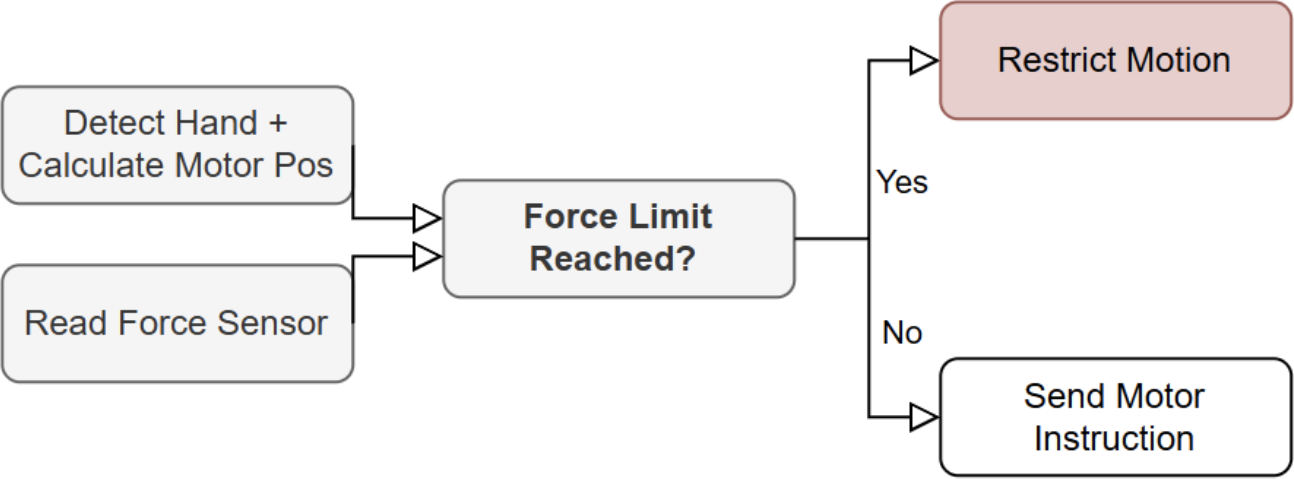
\includegraphics[width=0.5\linewidth]{figures/control_loop.png}
\caption{Force-aware grasp control loop. Target finger positions and live FSR
forces are constantly compared. If a finger's force exceeds the threshold,
motion is restricted and a red status LED lights; otherwise the servo command
is issued.}
\label{fig:block}
\end{figure}

\subsection{Mechanical Platform}
The hand is based on the open-source AmazingHand~\cite{pollen2025amazinghand}, a
four-fingered, fully 3D-printed design. Each finger is actuated by two Feetech
SCS0009 serial-bus micro servos (eight in total), giving four independently
controllable fingers.
We kept the original four-finger morphology, which is sufficient for force-aware
power and pinch grasps on our test objects and keeps the hand compact enough to
mount on a small arm. The fingertips were modified to host an FSR pad and to
route its leads back toward the palm (Figure~\ref{fig:mvphand}, left). The entire hand,
prototype board, and status LEDs are enclosed in a 3D-printed shell printed on
a Bambu Lab A1~Mini, with the electronics mounted on the back of the hand
(Figure~\ref{fig:enclosure}).

\begin{figure}[htbp]
\centering
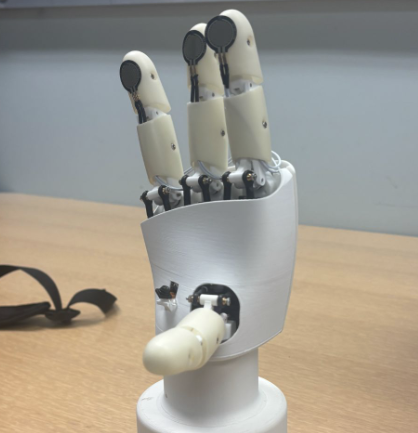
\includegraphics[height=4.3cm]{figures/mvp_hand.png}\hspace{0.03\linewidth}
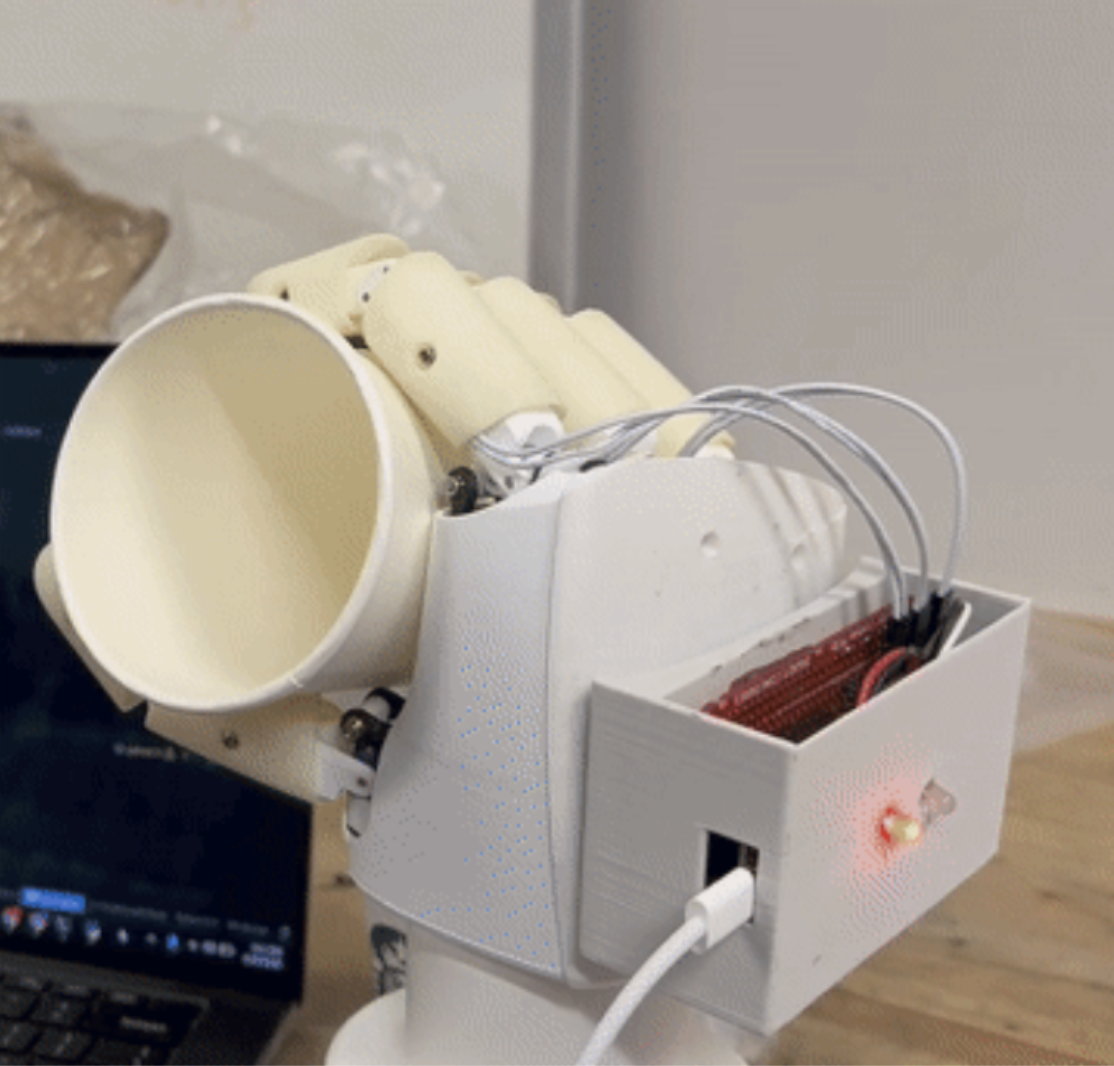
\includegraphics[height=4.3cm]{figures/closed_hand.png}
\caption{The Tactile Hand. Left: assembled on its base, with a force-sensing
resistor bonded to each fingertip and its leads routed back toward the palm.
Right: performing a force-aware grasp of a thin-walled cup, halting finger
closure the moment the measured fingertip force exceeds the safe threshold
(Section~\ref{sec:graspctl}).}
\label{fig:mvphand}
\end{figure}

\subsection{Sensing Electronics}
Each fingertip carries a Pololu \#2728 FSR. Because an FSR behaves as a
force-dependent variable resistor, we read it with a simple voltage divider: the
FSR is placed in series with a fixed reference resistor $R_\mathrm{ref}=48\,
\mathrm{k}\Omega$, and the ESP32-S3's 12-bit ADC samples the divider's midpoint,
$V_\mathrm{adc} = V_\mathrm{cc}\,R_\mathrm{ref}/(R_\mathrm{FSR}(F) +
R_\mathrm{ref})$. As applied force $F$ increases, $R_\mathrm{FSR}$ falls and
$V_\mathrm{adc}$ rises toward $V_\mathrm{cc}$; the ADC reports a raw count
$r \in [0, 4095]$. We use the ESP32-S3 for sending the data back to the host. The board is a protoboard hosting the
ESP32-S3, the four voltage dividers, and vertical 0.1-inch (2.54~mm) headers
for the FSR Dupont leads. Power comes from a 2S LiPo (7.4~V nominal) stepped
down to 5~V by a buck converter.

\begin{figure}[htbp]
\centering
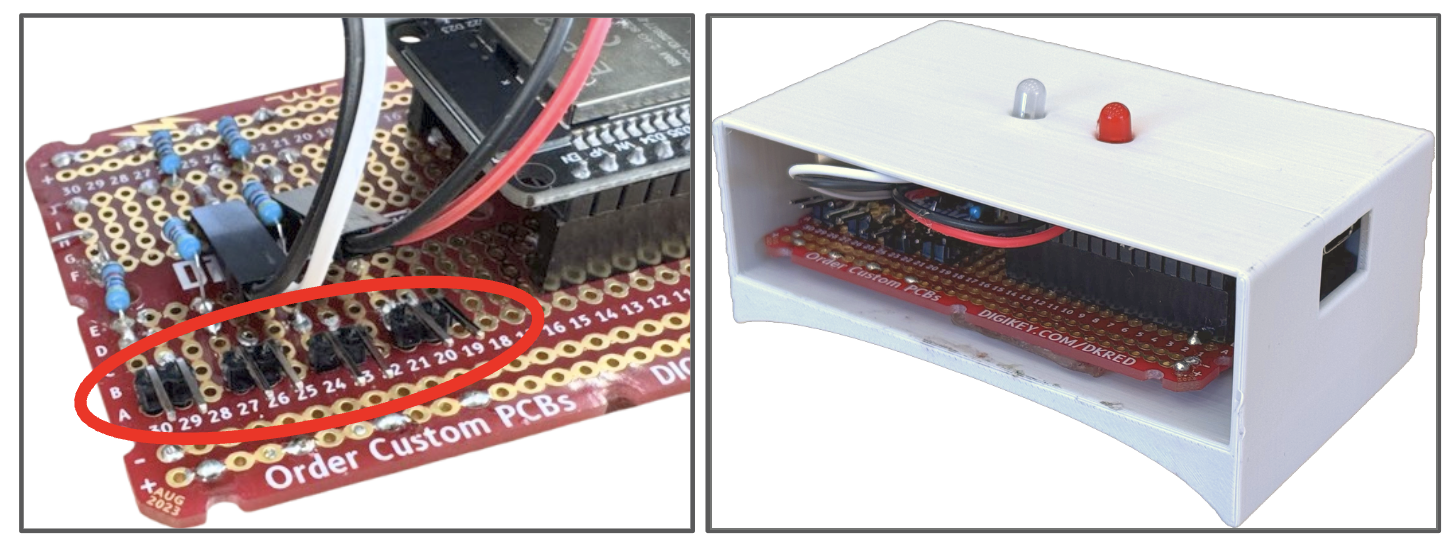
\includegraphics[width=0.72\linewidth]{figures/enclosure_circuit.png}
\caption{Custom ESP32-S3 sensing board (left) with the four FSR voltage-divider
channels highlighted, and the 3D-printed enclosure with status LEDs mounted on
the back of the hand (right).}
\label{fig:enclosure}
\end{figure}

\subsection{Firmware and ROS~2 Data Pipeline}
The firmware is built on the Arduino-ESP32 core. It samples the four ADC
channels at 100~Hz, applies the per-channel calibration described in
Section~\ref{sec:calibration} to convert raw counts to Newtons, and emits a
timestamped CSV line (timestamp followed by four force values) over a USB CDC
serial link at 115200~baud.

On the host, a ROS~2 (Humble, on Ubuntu) serial-bridge node parses the CSV
stream and publishes the calibrated forces on \texttt{/tactile/forces}. The same
node subscribes to \texttt{/servo/commands} and forwards target servo positions
to the ESP32 over the same serial link.

\subsection{Force Sensor Calibration}
\label{sec:calibration}
FSRs are strongly nonlinear and vary unit to unit, so raw ADC counts must be
mapped to physical force. We built a calibration rig that holds a sensor flat
and level, then stacked 3D-printed PLA reference weights on a loading plate so a
known mass rests on the active area (Figure~\ref{fig:calib}, left). For each load we
logged the ADC reading over serial. Sweeping a range of loads produced a set of
(raw count, force) pairs.

The FSR's count-to-force relationship is well captured by a power law,
\begin{equation}
F(r) \;=\; a\, r^{\,b},
\label{eq:powerlaw}
\end{equation}
which we fit by nonlinear least squares. Across seven loading points the fit
yielded $a = 1.07\times10^{-9}$ and $b = 3.16$, with a root-mean-square error of
17.1~g and a maximum error of 25.7~g (Figure~\ref{fig:calib}, right). Since
$1\,\mathrm{N}\approx102$~g-force, a 25.7~g worst case corresponds to roughly
0.25~N---comfortably within our 1~N accuracy target. The procedure is
documented and repeatable.

\begin{figure}[htbp]
\centering
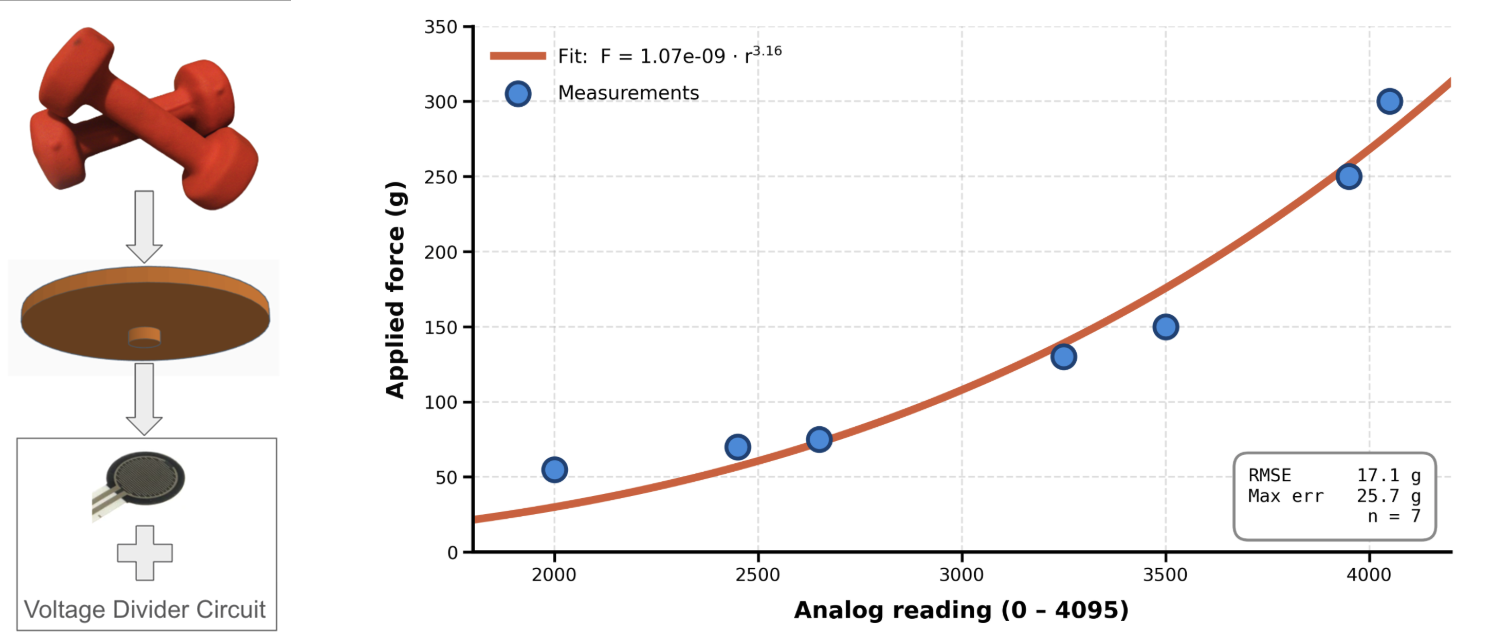
\includegraphics[width=0.9\linewidth]{figures/calibration.png}
\caption{Force-sensor calibration. Left: the calibration rig, a 3D-printed
loading plate on the FSR's active area loaded with stacked PLA reference weights
to apply a known mass. Right: a power-law model fit to seven stacked-weight
loading points maps raw ADC counts to applied force, with worst-case error
25.7~g ($\approx$0.25~N), well within the 1~N target.}
\label{fig:calib}
\end{figure}

\subsection{Force-Aware Grasp Control}
\label{sec:graspctl}
The grasp controller (Figure~\ref{fig:block}) runs on the host at the sensor
rate. A finger is driven toward a target curl by an open-loop closing
trajectory (during MVP demos) or by a teleoperation input. At every cycle the
controller reads that finger's calibrated force from \texttt{/tactile/forces}.
While the force is below the safe threshold $\tau$, the commanded position is
forwarded to the servo and the finger continues to close. The instant the force
crosses $\tau$, the controller freezes that finger's target (the ``restrict
motion'' branch) so it stops squeezing harder even though the nominal trajectory would
keep closing, and a red status LED (one of two indicator LEDs on the board)
lights to signal that the threshold has been reached. Release is triggered on
demand by commanding the fingers open. In practice this lets the hand wrap a
thin-walled paper cup and halt at its safe limit without buckling the wall
(Figure~\ref{fig:mvphand}, right).

\subsection{Vision-Based Hand-Pose Estimation}
To drive the hand from a human gesture we built a webcam pipeline on MediaPipe
Hands~\cite{zhang2020mediapipe} and OpenCV, which returns 21 hand landmarks in real time.
From the landmarks we estimate each finger's joint angles, reduce them to a
single normalized curl value in $[0,1]$ per finger, and map that value onto the
servo's angular range. The result is a four-element command vector published on
\texttt{/servo/commands}, so the robotic hand mirrors the operator's finger curl
live (Figure~\ref{fig:handpose}). Because the pipeline outputs the same
normalized curl interface used elsewhere, it is a drop-in alternative to the VR
input.

\begin{figure}[htbp]
\centering
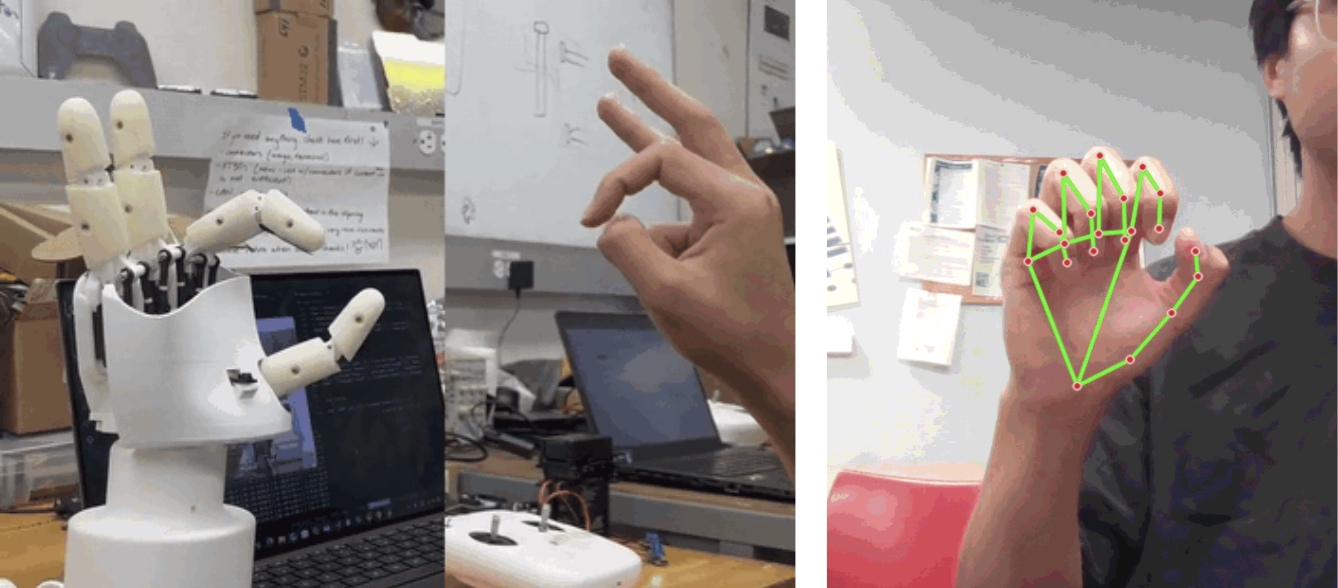
\includegraphics[width=0.68\linewidth]{figures/hand_pose.png}
\caption{Hand-pose mirroring. MediaPipe-based finger-pose estimation from a
webcam (right) is mapped to per-finger servo commands so the robotic hand
reproduces the operator's gesture (left).}
\label{fig:handpose}
\end{figure}

\subsection{Physics Simulation}
\label{sec:simsec}
We brought up the AmazingHand in the MuJoCo physics
simulator~\cite{todorov2012mujoco} by loading its
URDF/MJCF model and verifying that the simulated finger kinematics and curl
poses match the real hand. The simulation serves two
purposes: it is a safe sandbox for validating control logic before running it on
hardware, and it is the foundation for sim-to-real experiments. The main one is an
in-hand cube-rotation policy trained in simulation that we intend to
transfer to the real hand (Figure~\ref{fig:siminhand}, left), where the reality
gap~\cite{zhao2020sim2real} between simulated and physical FSR contact remains
the central challenge.

\begin{figure}[htbp]
\centering
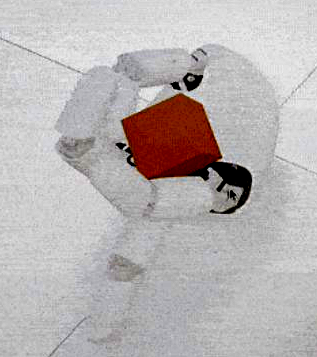
\includegraphics[height=3.6cm]{figures/sim_inhand.png}\hspace{0.03\linewidth}
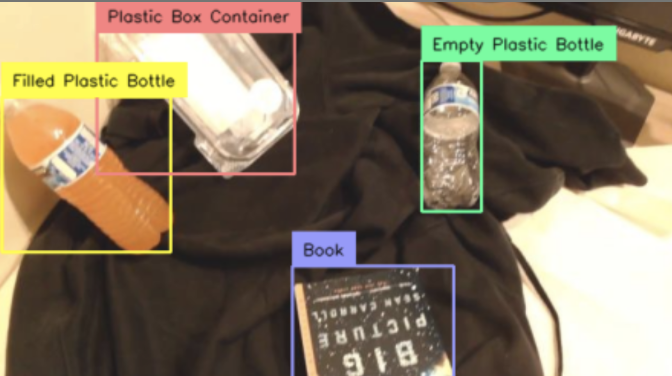
\includegraphics[height=3.6cm]{figures/yolo_detection.png}
\caption{Left: simulated in-hand manipulation. The AmazingHand model grasps a
cube in MuJoCo, the environment used to develop the in-hand cube-rotation policy
we intend to transfer to hardware. Right: vision-guided grip selection. A
fine-tuned YOLO26 detector recognizes each object and its class (e.g., filled
vs.\ empty plastic bottle), and the detected class selects a per-object
grip-force threshold the force-aware loop enforces (Section~\ref{sec:multiobject}).}
\label{fig:siminhand}
\end{figure}

\subsection{VR Teleoperation and Arm Integration}
\label{sec:vr}
Our final input modality is VR teleoperation. We initially built a Meta Quest~2
APK in Unity 2022.3 LTS from the
\texttt{unity\_ros\_teleoperation} framework~\cite{leggedrobotics_teleop} and
successfully streamed 6-DoF controller pose (position and orientation) into
ROS~2 on Ubuntu. While functional, the Quest~2 path was awkward to integrate
with our Python-based control stack. We therefore switched to Valve
Index controllers, read through OpenVR/\texttt{pyopenvr}~\cite{valve2024openvr},
which gave us a clean pure-Python interface and native per-finger capacitive
tracking. With the Index controllers, controller pose is published as a ROS~2
topic at interactive rates. The same per-finger capacitive sensing lets the
operator's finger motion drive the hand's fingers directly
(Figure~\ref{fig:vrindex}, left), so a single controller supplies both the 6-DoF wrist
pose and a per-finger curl signal on the shared \texttt{/servo/commands}
interface.

\begin{figure}[htbp]
\centering
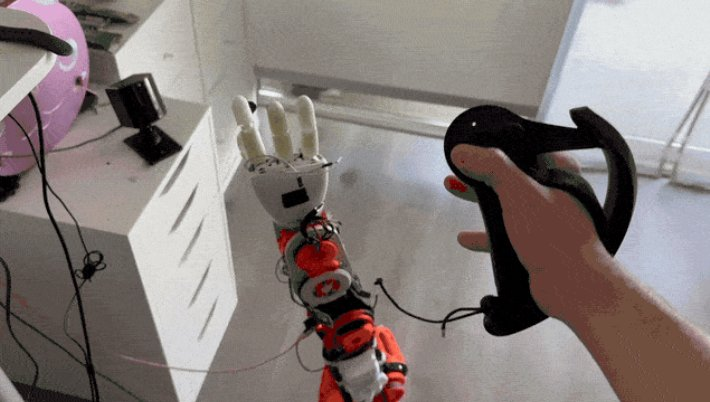
\includegraphics[width=0.4\linewidth]{figures/vr_index_hand.png}\hspace{0.02\linewidth}%
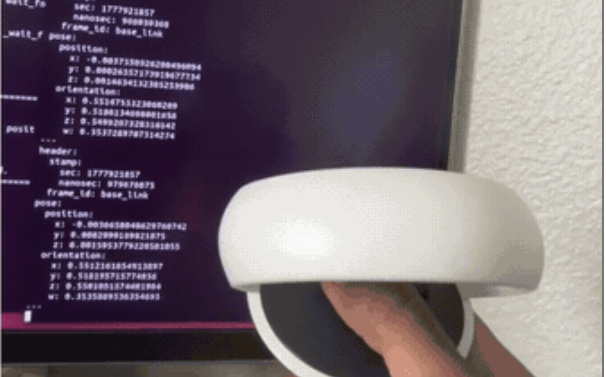
\includegraphics[width=0.368\linewidth]{figures/vr-demo.png}
\caption{VR teleoperation. Left: the Valve Index controller's native capacitive
finger tracking is streamed over ROS~2 to drive the robotic hand's finger curl
directly from the operator's hand. Right: the controller's 6-DoF pose drives the
ARCTOS arm end-effector through our framework (frame calibration, IK, and motion
smoothing), giving VR control of the arm-mounted hand.}
\label{fig:vrindex}
\end{figure}

To turn streamed pose into motion we mounted the hand on an open-source ARCTOS
robotic arm~\cite{arctos2024} and mapped controller pose to the arm's
end-effector. In the integrated platform the Tactile Hand is fixed to the
ARCTOS end-effector, and the whole arm-hand chain
is driven from the VR controller through the same ROS~2 stack used for the
standalone hand. We built a full end-to-end teleoperation framework for
the arm: moving an Index controller moves the ARCTOS arm's end-effector through
our ROS~2 pipeline, with controller-to-arm frame calibration, inverse
kinematics, and motion smoothing all in place, so the full chain from VR input
to physical arm motion is closed (Figure~\ref{fig:vrindex}, right).

\subsection{Teleoperated Force-Aware Grasping}
\label{sec:teleopgrasp}
Mounting the hand on the arm let us ask a sharper question than the scripted MVP
demo could: does the force-aware safety guarantee survive once a human is in the
loop and the grasp is no longer a fixed trajectory? To test this we kept the
force-aware controller of Section~\ref{sec:graspctl} active on the arm-mounted
hand while an operator teleoperated the arm to a fixed, thin-walled 3D-printed
cup and triggered a grasp. We ran the same teleoperated grasp under two
conditions: once with the force-aware controller enabled, and once with force
feedback disabled so the fingers simply close to a fixed curl; the operator
drives the same Index controller to the same cup in both runs.

The contrast is stark and repeatable. With force-thresholding enabled, each
finger halts at the cup's safe limit and the hand holds the cup with its wall
intact; with feedback disabled, the identical teleoperated motion drives
the fingers past the safe force and visibly buckles the cup wall
(Figure~\ref{fig:teleopcompare}). Because nothing changes between the two runs
except the force loop, the comparison isolates the contribution of the tactile
channel: the outcome flips from a clean hold to a crushed cup. The same safety
behavior that protected the cup in the scripted MVP holds up when a human is
driving the arm in VR.

\begin{figure}[htbp]
\centering
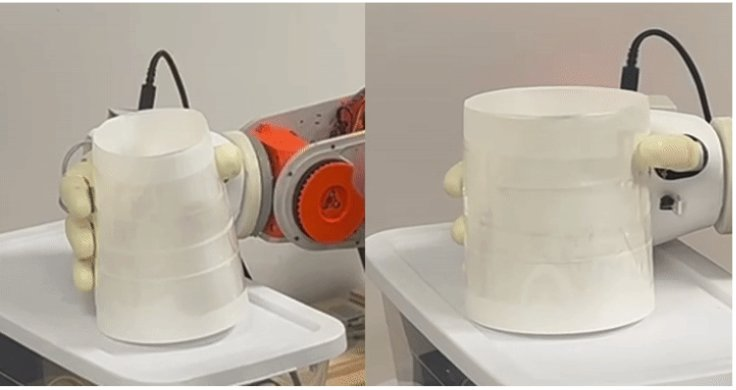
\includegraphics[width=0.65\linewidth]{figures/teleop_compare.png}
\caption{Teleoperated force-aware grasping. Under the same VR-teleoperated
motion, the force-blind grasp (left) crushes the thin-walled cup, while the
force-threshold grasp (right) holds it with the wall intact. Only the force loop
differs between the two runs.}
\label{fig:teleopcompare}
\end{figure}

\subsection{Multi-Object Force-Awareness and Vision-Guided Grip Selection}
\label{sec:multiobject}
A single hand-tuned threshold is enough for one known object, but a genuinely
useful hand must choose an appropriate grip force for whatever it is handed. We
extended the force-aware controller toward automatic, per-object grip selection
and exercised it on a small set of everyday objects that demand different
grips. The hardest case is an empty versus a filled plastic bottle, which look
nearly identical but differ sharply in weight and therefore in the grip force
needed to hold them without slipping or crushing.

Our pipeline recognizes the target in a webcam frame with a fine-tuned
YOLO26 object detector~\cite{ultralytics_yolo26}. We annotated a small custom
dataset of our objects (e.g., filled plastic bottle, empty plastic
bottle, plastic box container, and book) and fine-tuned YOLO26 on
it, giving real-time bounding-box detections with a class label per object
(Figure~\ref{fig:siminhand}, right). Each class maps to a hand-tuned target grip
force, with heavier or sturdier objects getting a firmer threshold and lighter or
more fragile ones a gentler threshold, and the detected class selects which
threshold the force-aware loop enforces. The detector changes only the
source of the target force; the downstream \texttt{/tactile/forces}
feedback path and the restrict-motion logic of Section~\ref{sec:graspctl} are
reused unchanged, which kept the addition lightweight.

This experiment also exposes a calibration limitation: FSRs respond differently
to off-axis and shear loading than to the normal loading used during calibration
(Section~\ref{sec:calibration}), so a misaligned grip reads a biased force. We
have begun characterizing each sensor's off-axis response and feeding it back
into the physics simulation (Section~\ref{sec:simsec}) to tighten the sim-to-real
match.

%=====================================================================
\section{Milestones}
\label{sec:milestones}
%=====================================================================
We targeted MVP completion by Week~6, with reach goals in Weeks~7--10.
Table~\ref{tab:milestones} lists each milestone and its final status.

\begin{table}[t]
\caption{Milestone status. All MVP-track items are complete; reach goals range
from complete to not completed, consistent with their deferred priority.}
\label{tab:milestones}
\small
\renewcommand{\arraystretch}{1.05}
\begin{tabularx}{\linewidth}{@{}Xll@{}}
\toprule
\textbf{Milestone} & \textbf{Target} & \textbf{Status} \\
\midrule
System design, board fabrication \& components & W2--W4 & Complete \\
Hand assembly, FSR integration \& firmware     & W3--W5 & Complete \\
FSR calibration to within 1~N                  & W4--W6 & Complete \\
Simulation bring-up of AmazingHand             & W3--W5 & Complete \\
Force-aware grasping closed loop               & W5--W6 & Complete \\
\textbf{MVP completion \& validation}          & \textbf{W6} & \textbf{Complete} \\
Hand-pose estimation pipeline (reach)          & W7--W9 & Complete \\
VR teleoperation: pose streaming, arm integration \& force-aware grasp (reach) & W7--W9 & Complete \\
Multi-object force awareness (reach)           & W8--W9 & Complete \\
Sim-to-real in-hand rotation (reach)           & W8--W9 & Not completed \\
Final paper, demo video, GitHub repo           & W9--W10 & In progress \\
\bottomrule
\end{tabularx}
\end{table}

\subsection{Mid-Quarter Revisions}
Our main mid-quarter revision was the VR hardware: we changed from the chartered
Meta Quest~2 to Valve Index controllers (Section~\ref{sec:vr}). We had a working
Quest~2 APK, but it was awkward to drive from our Python stack.

\subsection{What We Did and Did Not Finish}
All MVP deliverables were met, and the reach-goal outcomes are listed in
Table~\ref{tab:milestones}. Two items remain unfinished: the sim-to-real
transfer of the in-hand rotation policy (trained in simulation but not yet moved to hardware),
and finger adduction/abduction control (our curl interface captures flexion
only). Because reach goals were started only after the
Week~6 MVP, these gaps reflect the time available afterward, not a failure of the
core deliverable.

\subsection{Problems and Mitigations}
FSR nonlinearity and unit-to-unit variation threatened our 1~N target; the
stacked-weight calibration rig and power-law model brought worst-case error to
0.25~N. Quest~2 integration friction was resolved by switching to Valve Index. Mounting the hand
on the arm surfaced three further issues: ARCTOS wiring needed rework before the
arm drove reliably; off-axis fingertip loading during arm-driven grasps biases
readings relative to the normal-load calibration (we are characterizing this and
feeding it back into simulation, Section~\ref{sec:multiobject}); and the
read--decide--actuate loop has enough latency that the operator must close slowly
to avoid overshooting the threshold. The hand's wide palm limited its
reachability and made small objects hard to grasp, so we favored larger test
objects.

%=====================================================================
\section{Conclusion}
\label{sec:conclusion}
%=====================================================================
A robot hand that cannot feel how hard it is gripping is dangerous, and that
safety feature has been missing from affordable open-source hands. We presented
Tactile Hands, a sub-\$200 four-fingered robotic hand that adds calibrated
fingertip force sensing to the open AmazingHand platform and uses it to grasp a
fragile object without crushing it. Mounted on a VR-teleoperated arm, it
delivered our central result: under identical teleoperated motion, the
force-aware grasp holds a thin-walled cup while a force-blind grasp crushes it.

The significance of the work is accessibility: the most safety-critical sensing
capability of a robot hand, knowing its own grip force, can be added to a cheap,
reproducible platform without specialized hardware, and keeps working once the
hand is on a human-driven arm, lowering the barrier to safe manipulation research
and education.

Future work follows from our partial milestones: complete per-finger
calibration, grow the YOLO26 dataset toward learned weight-aware force targets,
carry the off-axis system-identification results into the simulator to close the
sim-to-real gap for the in-hand rotation policy, and refine the VR arm
teleoperation into reliable pick-and-place. All hardware designs, firmware,
calibration data, and software will be released publicly so that others can
reproduce a low-cost, force-sensing dexterous hand.

%=====================================================================
\bibliographystyle{ACM-Reference-Format}
\bibliography{references}

\end{document}